\documentclass[10pt,a4paper]{article}

\usepackage[margin=3cm]{geometry}
\usepackage[UKenglish]{babel}
\usepackage{enumitem}
\usepackage{calc}
\usepackage{fancyhdr}
\usepackage{graphicx}
\usepackage{multirow}
\usepackage[table]{xcolor}
\usepackage{float}
\usepackage{longtable}
\usepackage{parskip}
\usepackage{soul}
\usepackage[small,compact]{titlesec} 

\definecolor{titleColor}{RGB}{138,201,242}
\pagestyle{fancy}
\lhead{T Davies, A Fahie, A Fairbairn, A Free, J Mansfield, R Tucker, M Walker}
\chead{}
\rhead{GPIG-C}
\cfoot{\vspace{-0.6cm} \thepage}

\setlist{nolistsep} % Reduces lots of white space around lists

\renewcommand{\headrulewidth}{0.4pt} % Add rules below header
\renewcommand*{\thefootnote}{\fnsymbol{footnote}}

\begin{document}

\begin{center}
{\Large GPIG-C Interim Report}

Word count: @WORD_COUNT@
\unskip
\footnote{\textit{Using TeXCount, excluding\ldots}}

Friday, 14th February 2014
\end{center}

\vspace{0.3cm}
\rule{\textwidth}{0.4pt}


\section{Introduction}

\section{Glossary}

\begin{description}
	\item[HUMS] Health and usage monitoring system(s).
	\item[Customer] Thales. 
	\item[Consumer] The recipient organisation of the system.
	\item[(End) User] An individual or organisation using the system.
	\item[Client] A piece of computer hardware or software which accesses a
	              service made available by the HUMS system.
	\item[The System] The HUMS we are designing and developing.
	\item[Event] A point of interest flagged up by an analysis system, which
	             may result in a notification.
	\item[Data input client] Anything that provides data to the HUMS through
	                         the input interface.
	\item[Data output client] Anything that receives data from the HUMS
	                          through the reporting or notification interfaces.
	\item[Notification] A message sent by the system as a result of an event
	                    being fired.
	\item[Report] A message sent by the system as a result of a request from 				a user. 
	\item[HUMS Instance] One installation or occurrence of the system for a
	                     specific consumer.
\end{description}

\section{Requirements Refinement}

\section{System Architecture}
\subsection{Quality Attributes}
Quality attributes are defined in order to ensure the architectural decisions made when creating the system architecture not only provide the required functionality, but also produce a system meeting the expectations of all stakeholders. For example the system may be expected to meet certain security standards or availability levels. Explicitly defining these quality attributes before concretely designing a system allows for the correct tactics and patterns to be adopted in order to maximise the utility of important 
qualities.

When examining the HUMS non-functional requirements the following system quality attributes were identified:
	\begin{center}
	\textit{
		Availability, Performance, Modifiability, Security, Testability, Usability}
	\end{center}
Of these availability, performance, security and usability can be observed and measured, the others are unobservable however steps can still be taken to maximise their utility.
%Maybe go into more detail if space
Availability defines how ready the system is to be used, and is normally the percentage of downtime over a specified timeframe. The desired utility of the quality attribute within the HUMS, as defined by the non functional requirements, is  99.9\% per month. Since lack of availability is often linked to faults occurring, fault detection and recovery tactics, such as use of runtime exceptions, redundancy through backups and transactions, could be employed in order to achieve the desired level of availability. 

The performance of a system is normally measured by its latency and throughput. The HUMS is required to dispatch notifications through the notification generator after events have been triggered by the analysis controller, with a latency less than 5ms, the system is 
also required to be able to support multiple data output clients. Tactics such as reducing overhead though careful use of data structures and prioritising events can help reduce latency, at least for the most important events, defined by the end user. It may also be possible to add concurrency, such that multiple notification threads are used when demand for notifications and reports are high, reducing the bottleneck created at the notification generator.

Modifiability is one of the most important qualities of the HUMS, though not measurable, lack of modifiability can increase the cost and time taken to complete the project. The HUMS will initially be built to tackle a single domain, software, however, will in the future be required to work on embedded systems, mechanical systems, electrical systems and even people. In order to ensure these changes are as efficient as possible the initial system 
must be modifiable. Tactics that can be used to increase the modifiability of the system include using small modules within the system, decreasing the coupling between those modules and increasing the cohesion. In order to achieve low coupling  the HUMS uses interfaces between modules and restricts dependencies, such that the majority of modules can be swapped out without large changes to the overall system.

\subsection{System Views}
When designing the HUMS we identified four different views of of the system which must be documented:
\begin{description}
\item[Module View] The required software modules and relationships between them at a high level.
\item[Behavioural View] The flow of data and dynamic actions within the system.
\item[Deployment View] How modules are geographically positioned.
\item[Conceptual View] Class Diagrams, showing a concrete implementation of the functionality.
\end{description}

\subsection{Module View}
Having determined the quality attributes of the HUMS and the tactics which can be employed in order to achieve a high utility of these qualities a conceptual view can be formed. The conceptual diagram shown in figure \ref{fig:moduleDiagram} depicts the modules of the HUMS and the interactions between these modules at a high level.

%%TODO this diagram doesn't show the core or have a key
\begin{figure}[ht!]
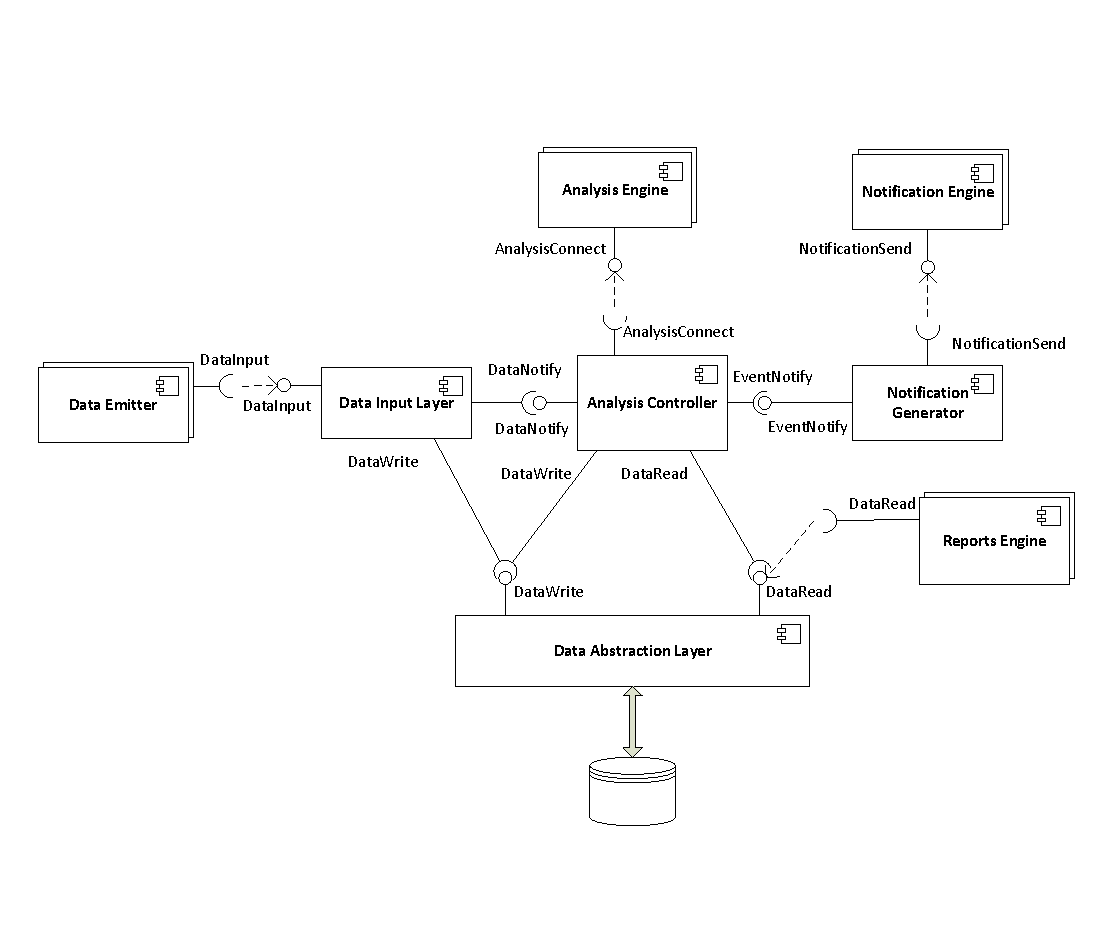
\includegraphics[width=15cm]{images/moduleDiagram.pdf}
\caption{The module diagram of the HUMS}
\label{fig:moduleDiagram}
\end{figure}

\begin{description}
\item[Data Emitter]  Sends data to the system core in a standard format, may be included within the HUMS or created by the end user.
\item[Data Input Layer] Receives data from a data emitter and sends it to the data abstraction layer. Alerts the analysis controller that new data was received.
\item[Data Abstraction Layer] Handles all interaction with the database, such that if the database was to be altered, only this layer would need to change.
\item[Analysis Controller] Alert the analysis engines when new data has arrived, pulling the required data from the data abstraction layer. If an analysis engine determines an event has occurred within the data then the analysis controller forwards that event to the notification generator
 \item[Analysis Engine] Analyses the data looking for trends, it a trend is found an event is returned to the analysis controller. Analysis engines may be included in the HUMS or created by the end user.
 \item[Notification Generator] Receives events from the analysis controller, defines an abstract notification and sends it to the appropriate notification engine.
 \item[Notification Engine] Receives an abstract notification from the notification generator and creates a concrete notification, for example an email or triggering a change in system behaviour. Notification engines may be included in the HUMS or created by the end user.
  \item[Reports Engine] Pulls data from the data abstraction layer and formats it into a report, for example a PDF or graph. Reports engines may be included in the HUMS or created by the end user.
\end{description}

\subsection{Behavioural View}
The module view shows how modules of the system are connected, however, does not fully represent the interactions between components and the dynamic actions of the system.
A behavioural view can be used to detail this information, showing the flow of data and events within the HUMS. Figure \hl{XXX} shows the behavioural model of the HUMS, detailing how the HUMS goes from receiving data from a data emitter to generating a notification.
%%Input Diagram WITH KEY

\subsection{Deployment View}
With view to deployment the HUMS needs to be tailorable, the core system may be running on the same hardware as the data emitter, it may also be geographically distant. Engines may all be on separate machines or may all be together. Figures \hl{XXX and XXX} show the most main scenarios for deployment of the HUMS, with a view that if the system architecture can perform under these situations, then it can perform under all others.

\hl{We also chose to look at deploying the system as a service....}
%% TODO talk about admin centre shizzle

\subsection{Conceptual View}
\subsubsection{Data Input Layer}
\subsubsection{Data Abstraction Layer}

The data abstraction layer, shown in figure \ref{fig:dataAbstractionPackage}, contains the following classes:
\begin{description}
\item [System Data Gateway] 
\end{description}

\begin{figure}[ht!]
\centering
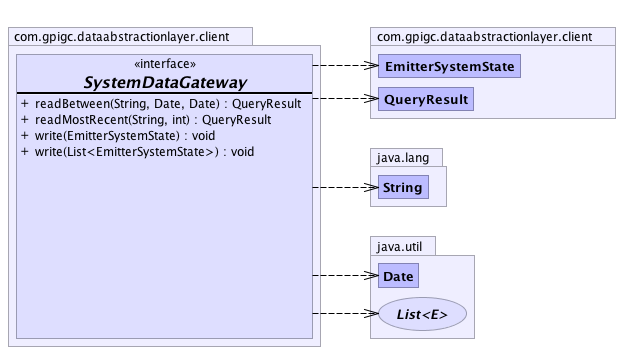
\includegraphics[width= 9.5cm]{images/DataAbstractionLayer/systemDataGateway.png}
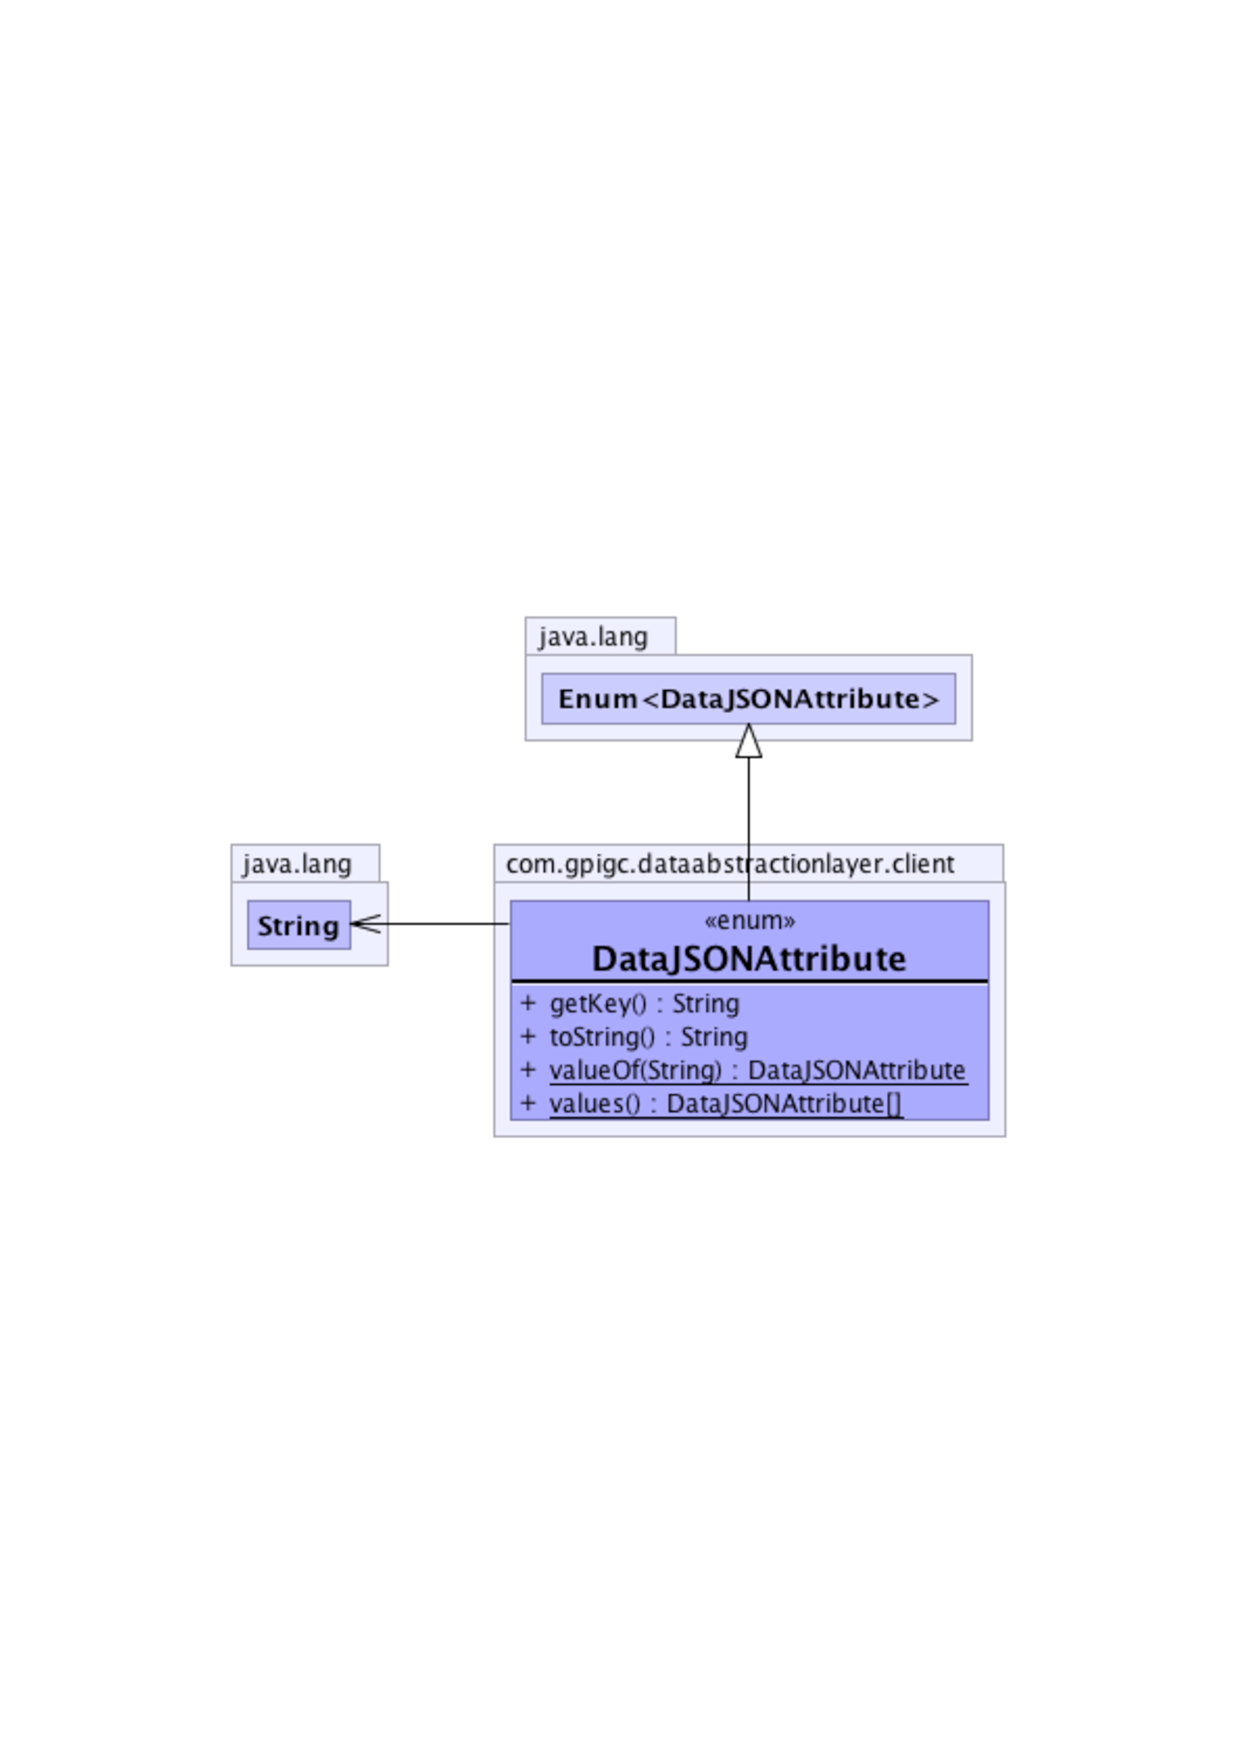
\includegraphics[width= 5cm]{images/DataAbstractionLayer/dataJsonAttribute.pdf}
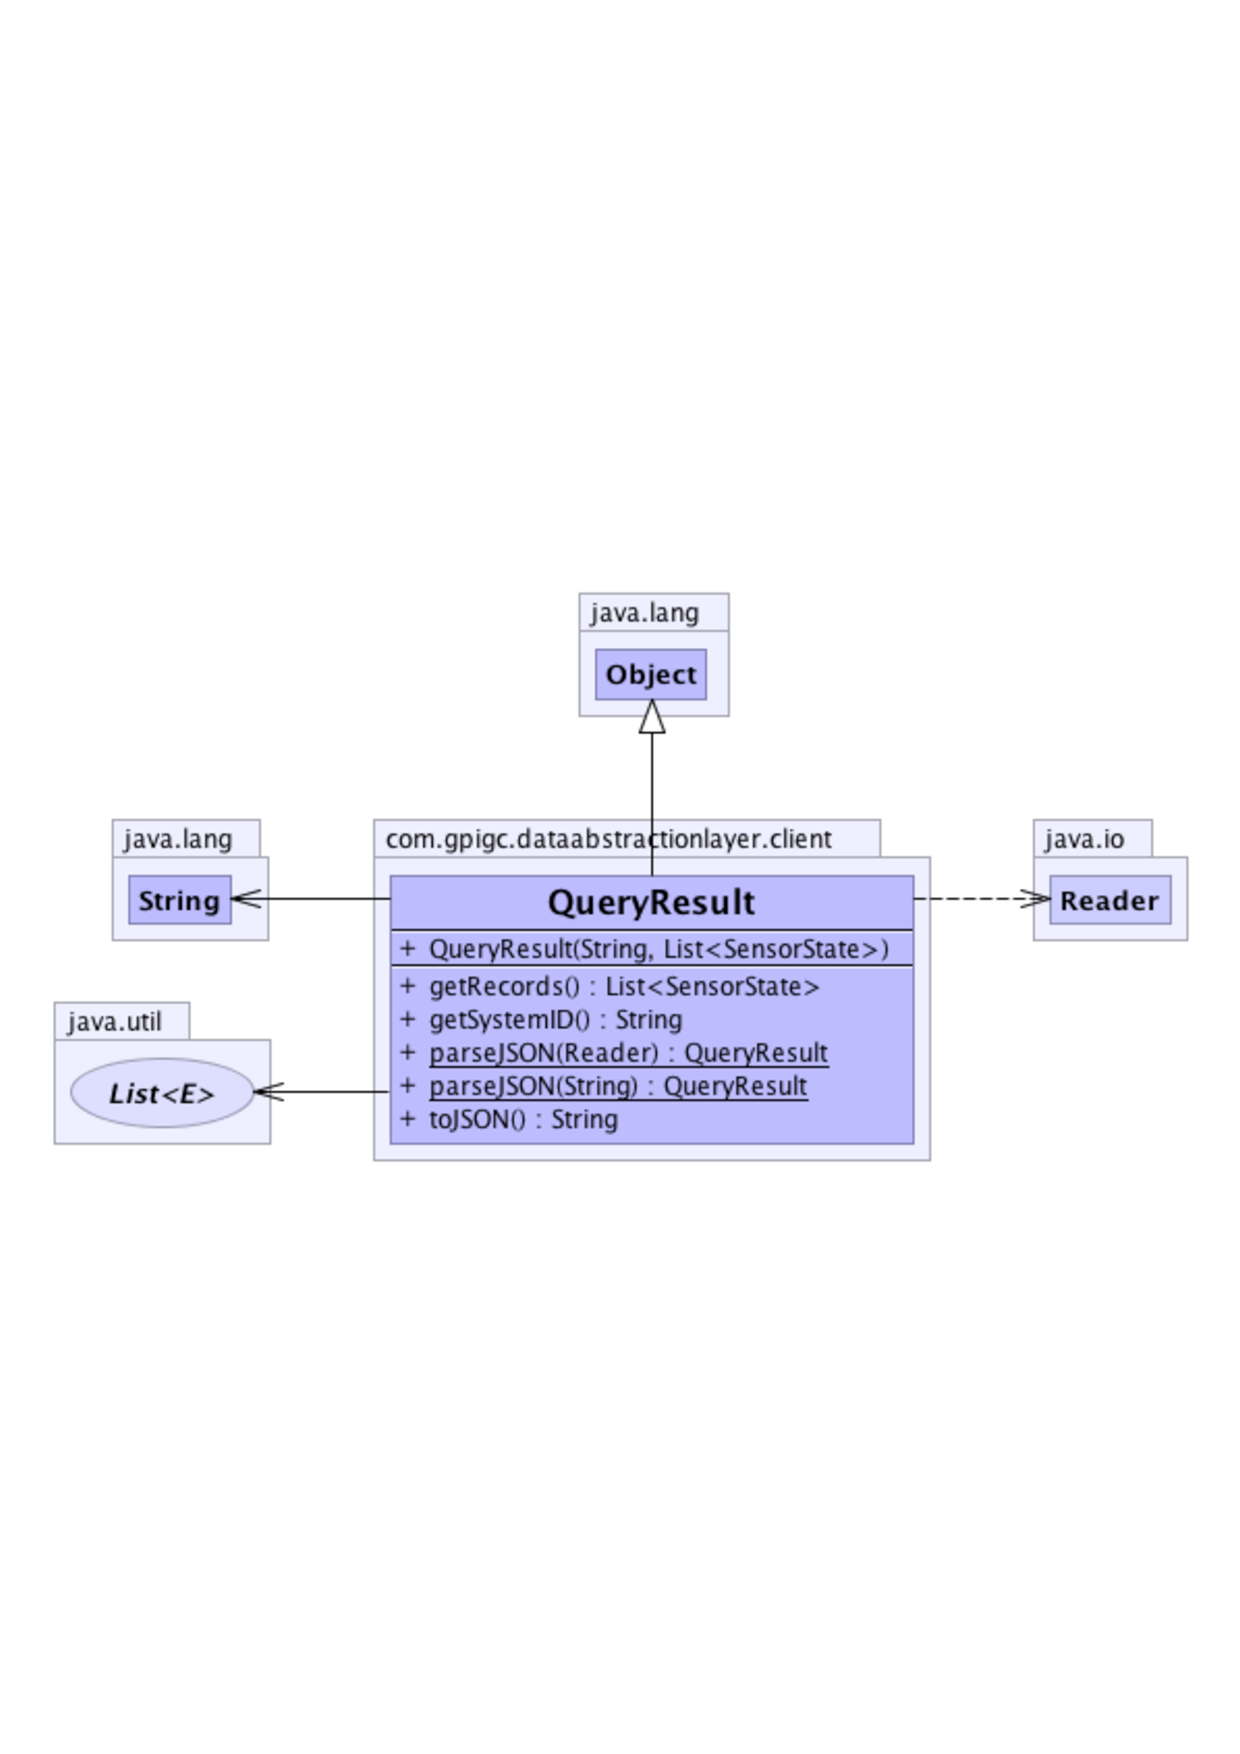
\includegraphics[width= 7cm]{images/DataAbstractionLayer/queryResult.pdf}
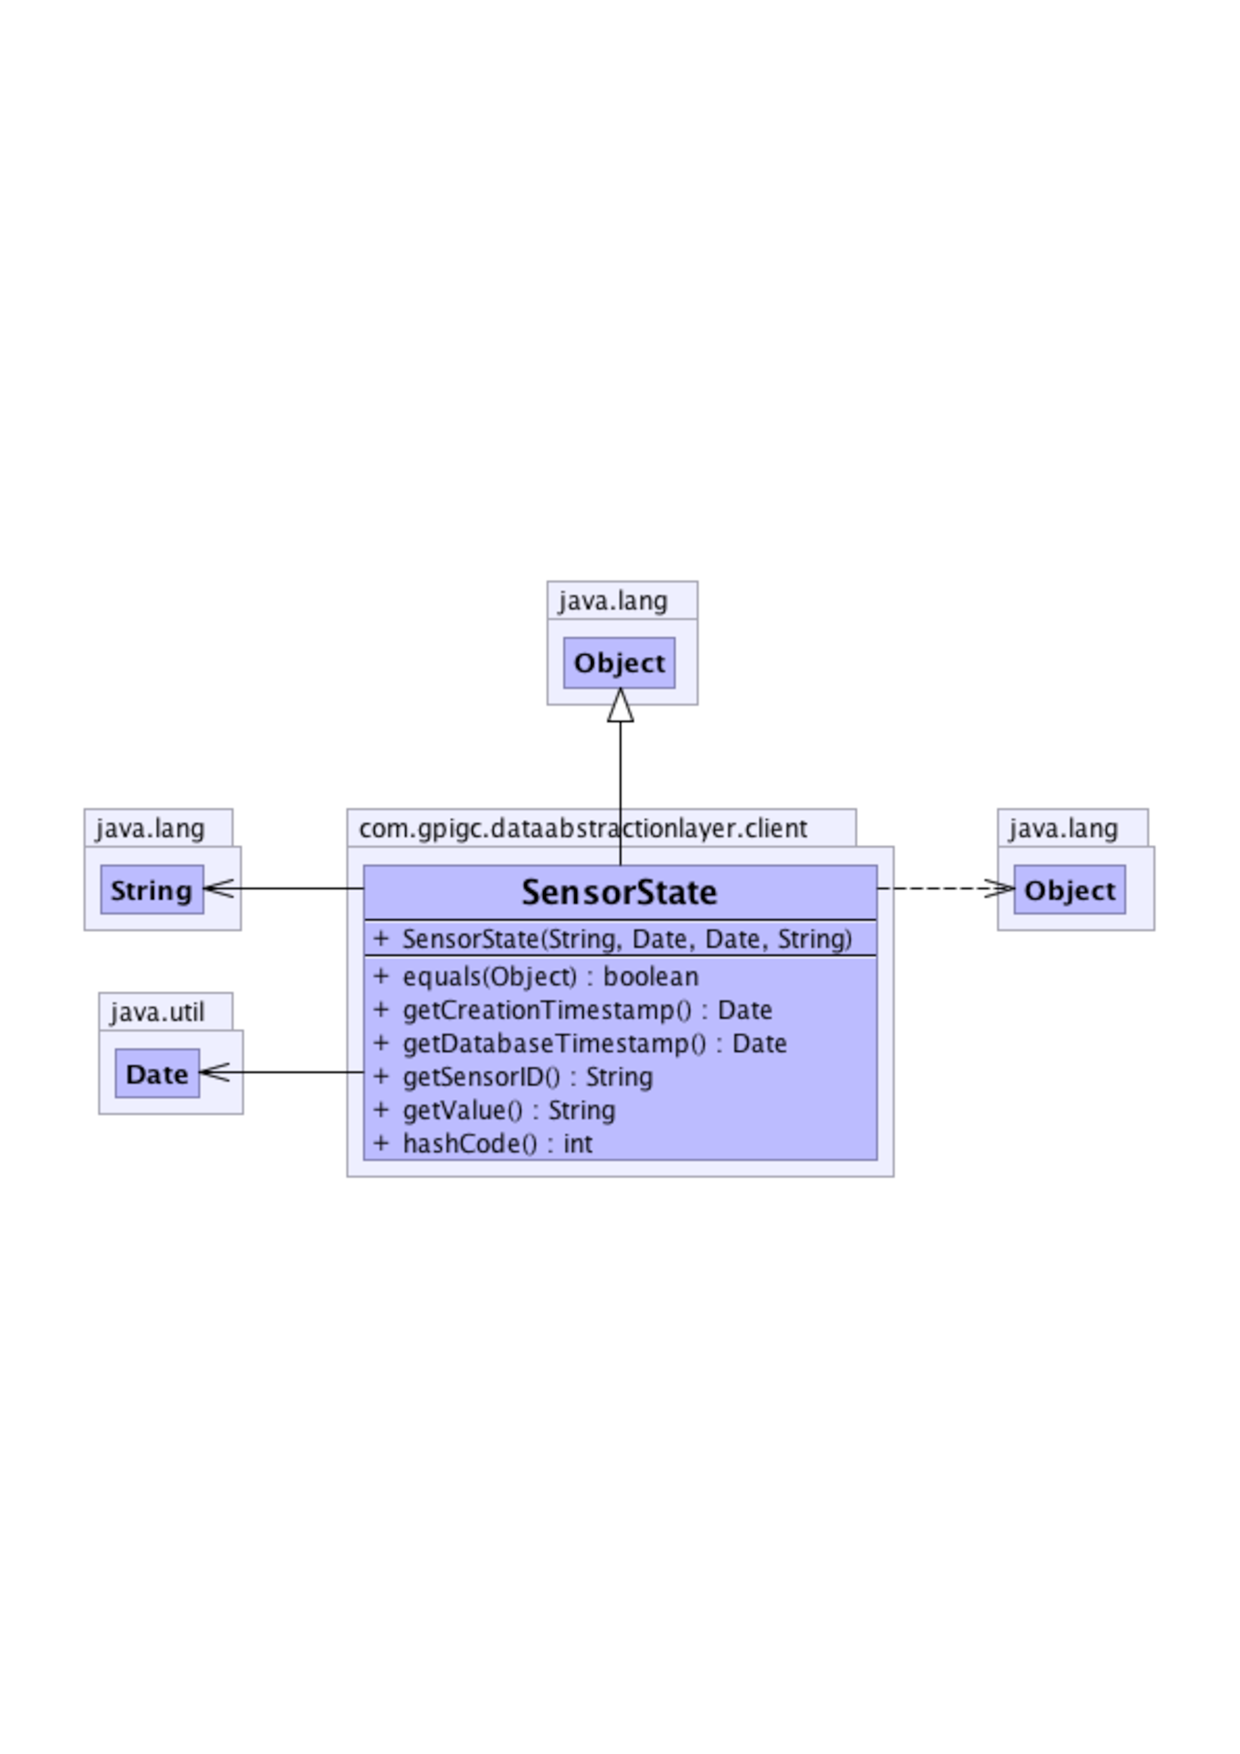
\includegraphics[width= 7cm]{images/DataAbstractionLayer/sensorState.pdf}
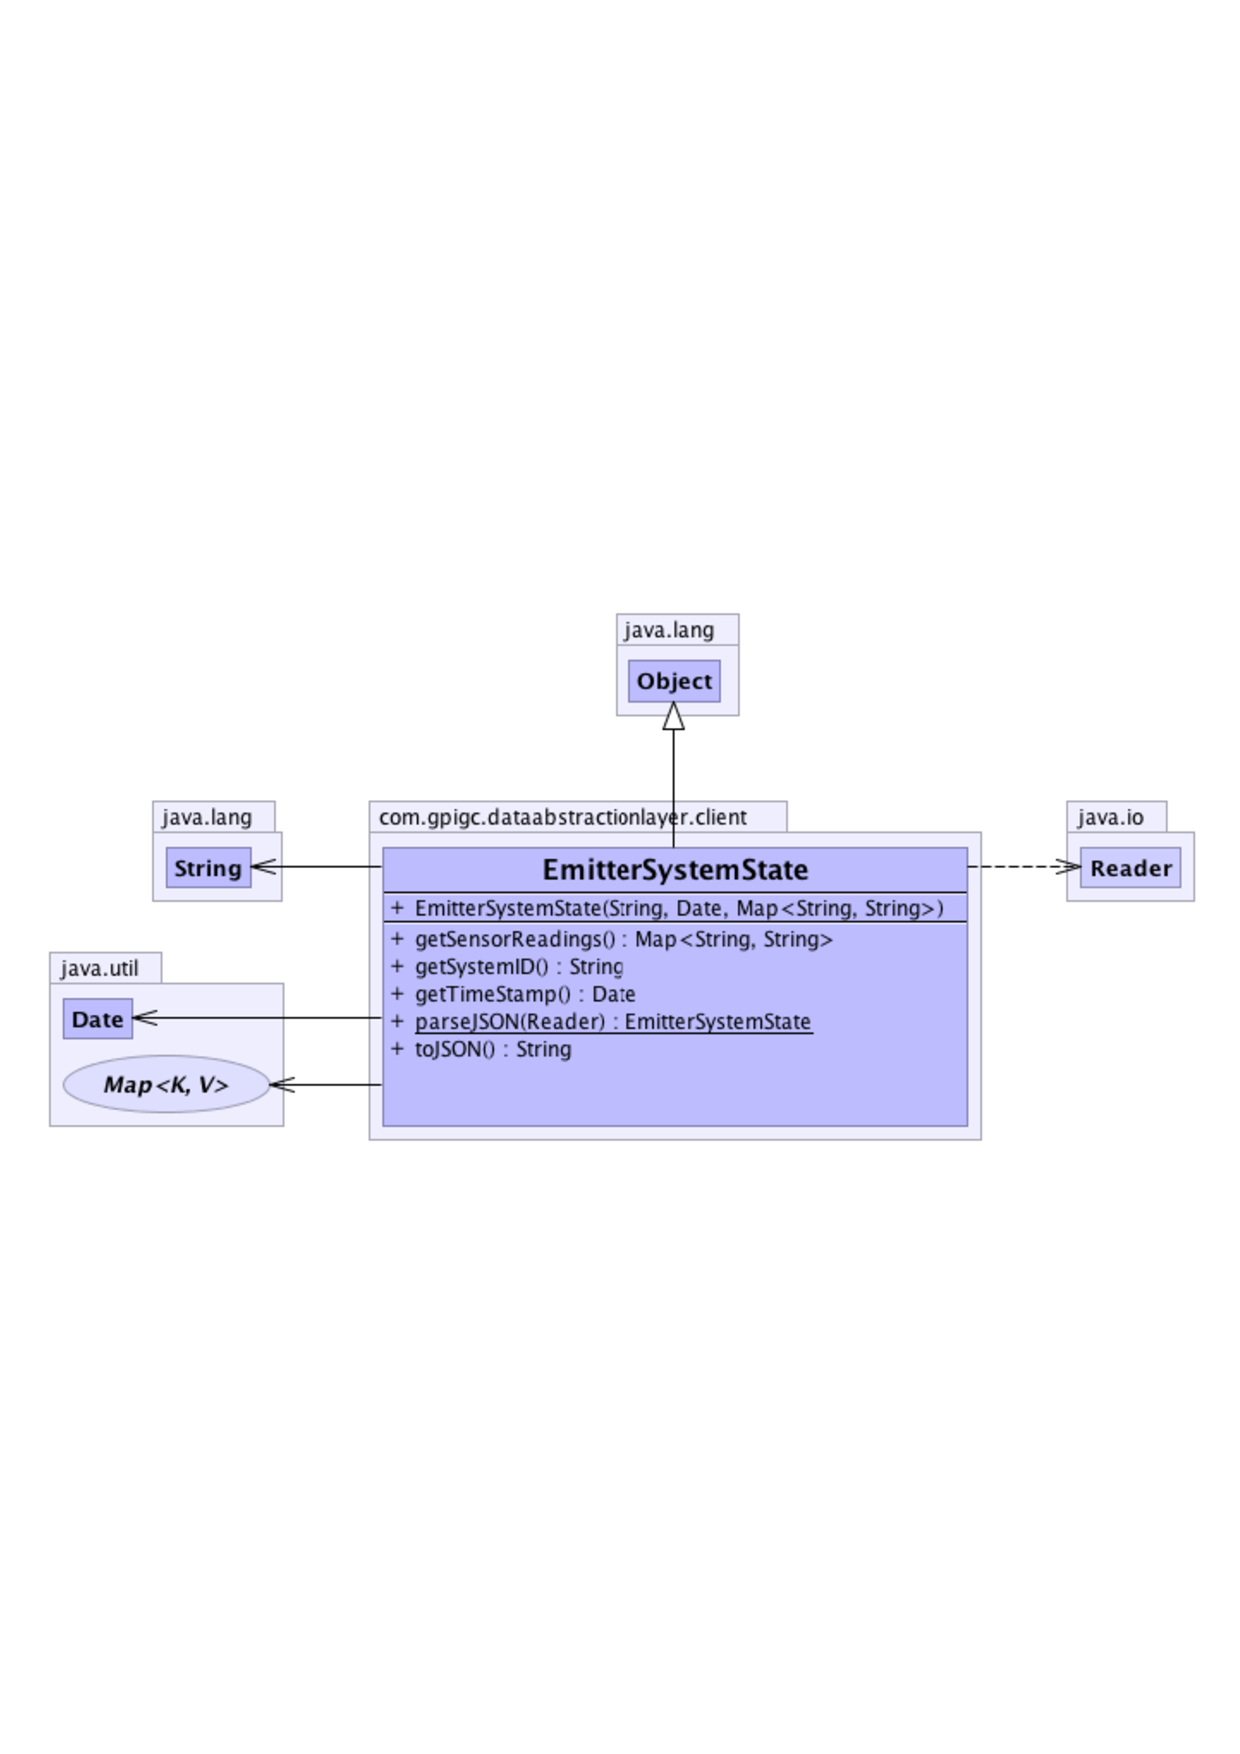
\includegraphics[width= 9cm]{images/DataAbstractionLayer/emitterSystemState.pdf}
\caption{Conceptual diagrams of the data abstraction layer classes, using UML 2 notation}
\label{fig:dataAbstractionPackage}
\end{figure}

\subsubsection{Analysis Controller}
\subsubsection{Notification Generator}

%%Class diagrams WITH KEYS

\section{Interim Prototype Implementation}

\subsection{Technologies}
We chose to develop the core of the HUMS prototype using Java, this does restrict its use, as the JVM is required, however, at this stage we do not see this as a problem since the underlying architecture of the system is transferable across languages.
All members of our team were familiar with the Java programming language and thus no time was spent having to learn or teach a new language. 
We did not impose a language restriction when developing the data emitter and various engines as the data being passed between them and the core is language independent, meaning end users are free, even with the prototype, to implement engines in any language they see fit. For the prototype we used Java and \hl{XXX} when creating the engines, languages team members are familiar with, allowing us to show off the versatility of the system.
We chose to use Google App Engine to host the database for the prototype, again wanting to show the versatility of the system, and how easily it can easily incorporate popular technologies. The prototype could easily be extended to work with other database technologies simply by implementing an interface within the data abstraction layer.

We created a prototype admin centre to show how the HUMS could be run as a service, allowing users to integrate their system, viewing and editing it online. The admin centre was developed using HTML, JavaScript and CSS in order to create a prototype realistically simulating the required behaviour.

We used Git for version control, allowing the entire team to contribute to the project simultaneously, and Google Docs for sharing notes, plans and meeting minutes when designing the prototype.
\subsection{Current Functionality}

\subsection{Testing}

\subsection{Evaluation on Test Application}

\section{Team Structure}

\section{Risk register}
A risk assessment has been performed as part of the initial report to ensure the team is aware of any problems which could later arise, and to provide a guide as to how to react when such problems occur. The hazards (risks) have been identified and classified based upon team members' past experiences in similar projects and group discussion. The areas these hazards impact were then analysed, as well as the probability of occurrence. These are then weighted so that we can identify the risks which are likely to have the greatest detrimental effect on the project. The likelihood score (LS), impact score (IS) and risk matrix score (RS) are listed in the table below.

\begin{longtable}[H]{| p{0.6cm} | p{2cm} | p{0.3cm} | p{2.6cm} | p{8.1cm} | p{0.7cm} |}
    \hline
    \cellcolor{titleColor}\textbf{Risk ID}   & \cellcolor{titleColor}\textbf{Risk}                                             &\cellcolor{titleColor}\textbf{LS}        & \cellcolor{titleColor}\textbf{Classification and Possible Impact}                                 & \cellcolor{titleColor}\textbf{Mitigation and Contingency} & \cellcolor{titleColor}\textbf{IS} \\ \hline                                                                                                                                                                                                                                                                                                                                                                                                                                                                                                                                
    \textbf{R.1}   & Short term loss of team members                  & 6       & \textit{Moderate}
\newline Deadline failure                                        
      &  The team can then reactively reallocate the team member's work across remaining team members. To aid with this, the team must proactively ensure that no work relating to the project is outside of team version control. Use of the scrum methodology proactively aids work reallocation, ensuring team members are aware of all assigned work. 
      & 18    \\ \hline
    \textbf{R.2}    & Long term loss of team members                   & 2 & \textit{Catastrophic}
\newline Deadline failure and low standard of deliverables 
    & If a team member is unavailable for an extended period, the team will react by notifying the customer and possible extending deadlines. The proactive procedures mentioned in \textbf{R.1} will also be followed to reduce the impact of this scenario.                                                                                                                                                                                                                                                                                            
    & 10    \\ \hline
    \textbf{R.3}     & Short or long term loss of resources             & 2 & \textit{Catastrophic}
\newline Deadline failure and loss of code base              
    & Proactive use of a source code repository, meaning code-base and history is decentralised. If the repository is lost, the data can be retrieved from the local repository copies and university backups.                                                                                                                                                                                                                                                                                                        
    & 10    \\ \hline
    \textbf{R.4}     & Team member under-performance                    & 3         & \textit{Major}
\newline Deadline failure and low standard  of deliverables            
    & Project plan must be feasible. The skills of the team as a whole, and individual team members must be proactively established early on and taken into account when assigning roles.                                                                                                                                                                                                                                                                                                                                                              
    & 12    \\ \hline
    \textbf{R.5}    & Mis-interpretation of requirements                & 3        & \textit{Major}
\newline Deliverables that are not valid                                        & 
    Requirements, design and implementation strategy must be proactively verified with the customer, this process is iterative, stopping when both customer and developers are content. Any changes to those requirements must result in re-negotiated deadlines.                                                                                                                                                                                                                                                                                    
    & 12    \\ \hline
    \textbf{R.6}    & Slow response to customer queries                & 3        & \textit{Major}
\newline Deadline failure and  low standard of deliverables         
    & Customer has assured a two working day response where possible. Further mitigation can be achieved by proactively communicating issues well in advance of deadlines.                                                                                                                                                                                                                                                                                                                                                                            
    & 12    \\ \hline
    \textbf{R.7}     & Failure to produce required system functionality & 2 & \textit{Catastrophic}
\newline Wasted time and loss of marks                        
    & Customer verification of requirements can counteract this risk. System testing, to ensure all agreed upon requirements are met, will also reduce this risk.                                                                                                                                                                                                                                                                                                                                                                                      
    & 10    \\ \hline
    \textbf{R.8}     & Missing internal team deadlines                  & 5            & \textit{Moderate}
\newline Project falls behind due to missing dependencies                     
    & Perform critical path analysis to identify tasks which will take the longest time and which are a prerequisite to others. A greater team effort can then be assigned to these areas if it seems likely to miss a deadline or halt progress elsewhere.                                           
    & 15    \\ \hline
\end{longtable}


The likelihood score defines probability of something occurring. Utilising
\textit{Kents Words of Estimative Probability}\cite{kent1966strategic}, with
`certain' weighted $7$ and `impossible' weighted $1$.

\begin{longtable}[H]{c c l | c | c | c | c | c | }
		\cline{4-8}
		& & & \multicolumn{5}{ c| }{Impact Score (Least$\rightarrow$Most)} \\ \cline{4-8}
		& & & 1 & 2 & 3 & 4 & 5 \\ \cline{4-8}
		& & & Negligible& Minor & Moderate& Major & Catastrophic \\ \cline{1-8}
		\multicolumn{1}{ |c }{\multirow{7}{*}{Likelihood Score}} & \multicolumn{1}{ |c| }{7} & Certain & 7 & 14 & 21 & 28 & 35 \\ \cline{2-8}
		\multicolumn{1}{ |c }{} & \multicolumn{1}{ |c| }{6} & Almost certain & 6 & 12 & 18 & 24 & 30 \\ \cline{2-8}
		\multicolumn{1}{ |c }{} & \multicolumn{1}{ |c| }{5} & Probable& 5 & 10 & 15 & 20 & 25 \\ \cline{2-8}
		\multicolumn{1}{ |c }{} & \multicolumn{1}{ |c| }{4} & Chances about even & 4 & 8 & 12 & 16 & 20 \\ \cline{2-8}
		\multicolumn{1}{ |c }{} & \multicolumn{1}{ |c| }{3} & Probably not & 3 & 6 & 9 & 12 & 15 \\ \cline{2-8}
		\multicolumn{1}{ |c }{} & \multicolumn{1}{ |c| }{2} & Almost certainly not & 2 & 4 & 6 & 8 & 10 \\ \cline{2-8}
		\multicolumn{1}{ |c }{} & \multicolumn{1}{ |c| }{1} & Impossible & 1 & 2 & 3 & 4 & 5 \\ \hline
\end{longtable}

\begin{table}[h!]
	\begin{tabular}{ | p{2cm} | p{4cm} | p{10cm} | }
		\hline
		\textbf{Score}&	\textbf{Risk Level}&	\textbf{Recommended Response}	\\ \hline
		\textbf{23-35}&	HIGH&	Mitigation plan is required. Immediate action is required.	\\ \hline
		\textbf{11-22}&	MEDIUM&	To be included in the action plan and reviewed.	\\ \hline
		\textbf{0-10}&	LOW&	Included in action plan in limited scope. Minimum review.	\\ \hline
	\end{tabular}
\end{table}


\section{Customer communication}
As we are, and were, aware that the customer may not be able to respond to communications rapidly. We have taken a proactive approach to communications. For each response from the customer, we organised group meetings within two days to discuss the feedback issued and to collaborate on any improvements to our solution we could make based upon the customer communication. We have previously highlighted in the document, in the relevant section, some of the feedback which we have taken on board from the previous assessment feedback. So this section is dedicated to communication in the form of emails since the previous assessment.

The feedback from the customer (?/? Date ??) suggested that our concept of SaaS and PaaS is interesting, and as such we have developed this idea to include the application to various usage scenarios. Furthermore, the feedback was that the website we presented in this communication did not sufficiently explain what the HUMS concept was to the potential consumers accessing our HUMS SaaS website. Therefore, we have added a section explaining how the HUMS system works and how it can be conveniently applied to various applications which are relevant to the consumer.

\vfill
\bibliography{report-refs}
\bibliographystyle{IEEEtran}
\end{document}
